\label{Elecciones}
\chapter{Análisis Elecciones}
\section{Elecciones Internacionales}
\subsection{EEUU}
En los años 50 y 60 se utilizaron boletas de tarjetas perforadas, pero este sistema generó mayores problemas al momento del escrutinio como por ejemplo, abolladuras en el papel, se consideraban válidas las marcas sólo si todos los presentes estaban de acuerdo. Las papeletas marcadas con pluma, perforadas más de una vez, perforadas de forma ambigua (por ejemplo, en la línea entre dos partidos) o sin perforación se consideraban votos inválidos.
Como solución a los problemas evidentes de los sistemas de tarjetas perforadas, comienza el auge de los dispositivos de registro electrónico directo de votos (DRE). El uso de dispositivos de votación en EEUU cobró especial relevancia a partir del año 2000, luego de las elecciones presidenciales en donde un gran número de votos no fueron registrados apropiadamente.  \newline
Actualmente, en los distintos estados se emplean diferentes sistemas, que a menudo son utilizados combinadamente. Sin embargo, existen debates sobre los dispositivos utilizados, y existen causas judiciales en muchos estados respecto a su uso. Como ejemplo en el estado de Pensilvania se produjeron varios problemas en el equipo de votación electrónica utilizados en Noviembre del 2019, generando suficiente desconfianza en el sistema de votación para las elecciones del 2020. Otro caso es el ocurrido en Nueva Jersey en el que los resultados fueron inmediatos pero el total de votos emitidos no coincidía con la suma de los votos emitidos por partido. \cite{eleccionesEEUU}.
En 2002 se aprueba la ley federal Help America Vote Act., que establece un organismo de control denominado Eleccion Assistance Commission (EAC). El EAC conforma un comité técnico para delinear recomendaciones guías para los sistemas de votación, en aspectos de seguridad, testing de usabilidad y establecimiento de estándares y método de prueba para sistemas de votación electrónica. En 2007, la EAC comenzó el proceso de certificación de equipamiento de voto electrónico. Además esta comisión lleva registro de distintos problemas reportados sobre los dispositivos que se usan en la actualidad (Voting System Reports Collecction, 2017) \cite{problemasReportados}.

\subsection{Irlanda}
La primera propuesta de voto electrónico en Irlanda se realizó en 1998 y en el 2000 se introdujo la legislación que permitió el voto eletrónico. Para el 2002, se hicieron las primeras pruebas piloto con el objetivo de extenderlo al resto del pais. Pasaron unos meses para que un informe confidencial del Ministerio del Interior irlandés se filtrara a la prensa: allí se aseguraba que la integridad del proceso electoral no estaba garantizada. Entre otras fallas, el memorando interno que tomó estado público destacaba la posibilidad de que un software malicioso sencillo de programar pudiera generar una pantalla falsa en la máquina para hacer votar incorrectamente al elector. A pesar de este manto de sospecha sobre el sistema, el gobierno irlandés avanzó con el plan de implementación para las eleciones locales y europeas de 2004. Entonces creó la Comisión Independiente de Votación y Escrutinio Eletrónico para que examinara el sistema propuesto. La comisión emitió un informe en el que sostuvo que puede recomendar la utilización del sistema de voto eletrónico pero que, no podía garantizar la seguridad del voto y la rigurosidad del escrutinio. El gobierno no dio marcha atrás con el sistema pero lo puso en suspenso. La inversión que hizo Irlanda en el sistema fue uno de los argumentos principales de las autoridades para no descartar el sistema. Como resultado se registró 52 millones de libras iniciales que se le pagaron a Nedap, y se agregaban los costos de mantenimiento y de actualizacion del sistema (calculando en 700.000 euros anuales y 20.000.000 por única vez).\newline
Finalmente, el 23 de abril de 2009 el entonces ministro anunció que quedaba descartado el sistema de voto electrónico, en base al alto costo de mantenimiento y actualización y la insatisfacción y sospechas que generó entre los electores. En 2019 se realizó una encuesta al público sobre el uso de elecciones electrónicas consiguiendo un 50\% de aceptación. \cite{eleccionesIrlanda}
\subsection{Holanda}
En el 2008 (un año antes que en el caso irlandés) el gobierno de Holanda había tomado la misma decisión: abandonar el sistema de voto electrónico que había comprado a una empresa local, Nedap. La batalla contra el voto eletrónico en Holanda fue un grupo de activistas informáticos denominado "We don't trust voting computers". Este grupo además de presentaciones judiciales, realizaron una demostración pública en un programa de televisión de las múltiples formas en las que se podía acceder y tomar el control de las máquinas Nedap sin demasiado esfuerzo. En menos de cinco minutos, lograron correr su propio software en una máquina de la empresa y repartir votos de acuerdo a sus preferencias, engañando al elector que utilizaba la máquina. Hasta el día de hoy, Holanda mantiene el sistema de voto por medio de boleta de papel.\cite{netherlands}

\subsection{Estonia}
En las elecciones municipales del 2005, Estonia se convirtió en el primer país del mundo en probar el voto por Internet, remoto. El sistema permite optativamente votar por Internet desde un lugar remoto, la identificación se hace a través del documento nacional de identidad que es una tarjeta inteligente; el voto por Internet es previo al día de la votación dejando al elector modificar su voto las veces que desee, tomandose como válido el último voto. En 2005, casi el 2\% utilizó el mecanismo de voto por Internet y fue creciendo hasta llegar al 30\% de la población en 2015. Las pocas garantías que ofrece sobre el carácter secreto del voto es una de las principales críticas que recibe este sistema. Los expertos consideraron que se debía suspender la aplicación de esta forma de votación, pero las quejas fueron rechazadas por el Comité de Voto por Internet del país y, en 2015, Estonia celebró sus elecciones con el sistema de voto por Internet.\newline

\subsection{Alemania}
A partir de 1998 comenzó a utilizar dispositivos electrónicos de voto (DRE Nedap utilizados en Holanda), comenzando con pruebas pilotos en Colonia y sucesivamente adoptados en distintas ciudades, y generalmente bien aceptadas por la ciudadanía, hasta 2005. En ese año, un par de ciudadanos presentaron una causa ante la Corte Constitucional Alemana, alegando que el uso de máquinas de votación electrónica es inconstitucional y que, dado que son vulnerables, los resultados de las presidenciales de 2005 no son confiables. Un fallo de esta corte dictaminó que el uso de las máquinas Nedap es inconstitucional, aunque no prohíbe el uso de cualquier dispositivo electrónico, sino que requiere que los mismos sean transparentes. Hoy Alemania usa la boleta única en papel.

\subsection{Brasil}
En 2002 implementó una elección a escala nacional utilizando unos 406.000 dispositivos electrónicos (DRE) en la cual más de 100 millones de votantes emitieron su sufragio. Los reportes de testing de seguridad públicos en 2012 muestran que existen problemas técnicos severos en los dispositivos utilizados. Entre los problemas más relevantes se señalan la inadecuada protección del secreto del voto, el uso inapropiado de encriptación y algoritmos de criptografía obsoletos, modelos de ataques inadecuados centrados en atacantes externos cuando los ataques internos presentan un riesgo mucho mayor, adopción de un proceso de desarrollo de software defectuoso y verificación de integridad insuficiente.



\section{Elecciones Las Grutas}
El 16 de diciembre de 2007 se utilizaron 4 urnas electrónicas de la firma Altec Sociedad del Estado (Rio Negro) en la localidad de Las Grutas (Argentina). Durante la jornada electoral, ocurrieron casos donde la urna no habilitaba al votante siendo que en el padrón en papel figuraba, siendo un claro atentado contra el secreto del voto. Otro de los problemas fueron máquinas que se trababan y al trabarse el papel utilizado dejaba en evidencia la elección del votante. La utilización de estas urnas electrónicas se implementó a pesar que el 10\% de los habitantes del lugar elevaran al superior tribunal de justicia la no obligatoriedad de este sistema. \cite{eleccionesLasGrutas}

\section{Elecciones Neuquén}
El 10 de Marzo de 2019, Neuquén realizó la elección para gobernador y vicegobernador por medio del sistema de boleta electrónica, con ciertas mesas con menor frecuencia pública a través del sistema tradicional en papel. Se utilizaron máquinas como se muestra en la figura \ref{fig:maquinasBUE}, el cual eran manipuladas directamente por el votante, imprimiendo su votación sobre una boleta electrónica utilizando un chip que luego es usado para el escrutinio de cada mesa. El proceso de votación se conforma de los siguientes elementos:

\begin{center}
  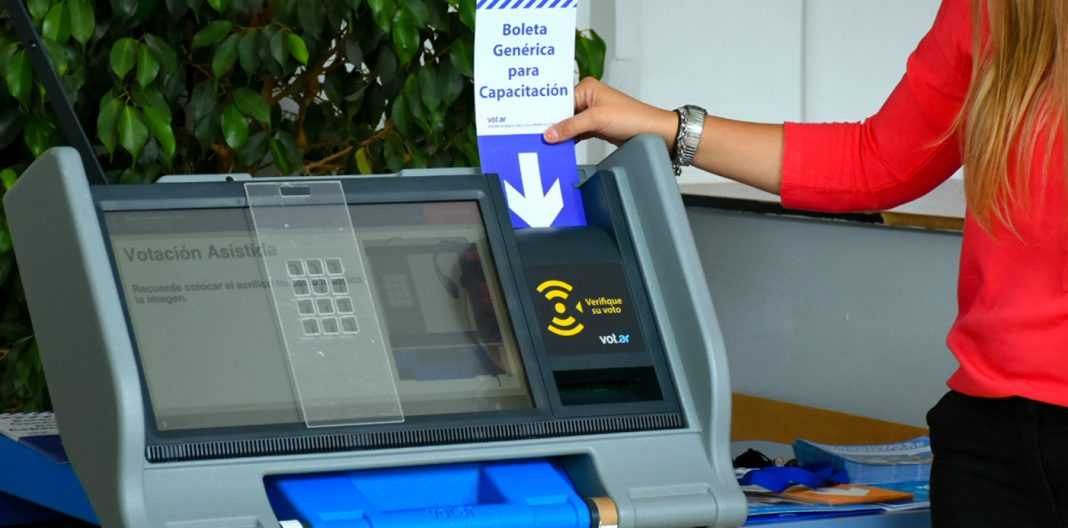
\includegraphics[scale=0.4]{Maquina_BUE.jpg}
  \caption{Máquina utilizada en las elecciones de Neuquén}
  \label{fig:maquinasBUE}
\end{center}[h!]

\begin{itemize}
    \item Votación utilizando la máquina electrónica.
    \item Conteo utilizando la maquina electrónica y las boletas electrónicas.
    \item Envío de datos de las escuelas con la máquina electrónica utilizando el certificado generado de cada escrutinio de la mesa.
    \item Resultados provisorios
\end{itemize}

\newline Sobre estas elecciones se obtuvieron los siguientes datos:
\begin{itemize}
    \item 497.448 neuquinos estuvieron habilitados para votar, de los cuales se contabilizó una participación del 78.44%
    \item 1.504 mesas distribuidas en 283 escuelas, de las cuales 191 trabajaron con el sistema BUE (Boleta Única Electrónica), 86 con el sistema tradicional de papel y 6 escuelas tuvieron ambos sistemas
\end{itemize}

\subsection{Fiscalización Virtual/Informático para elecciones en Neuquén}
En Febrero de 2019 se participó como fiscales informáticos para Unidad Ciudadana en las elecciones provinciales de Neuquén para ese mismo año. La misión de un fiscal es verificar y auditar el sistema a utilizar en la emisión de sufragio, las boletas y el sistema de recuento provisorio. El objeto es detectar cualquier situación que pudiera poner en riesgo la transparencia o la equidad en los comicios, o llevar a confusión al elector. Para llevar adelante este proceso la Justicia Electoral de Neuquén convocó a diferentes agrupaciones políticas para auditar la quema de DVDs y la prueba de transmisión. Estos DVDs son el medio para iniciar y habilitar las máquinas para su posterior uso en la votación, y la prueba de transmisión se ejecuta sobre una máquina que contiene los mismos componentes que las máquinas de votación pero utiliza otro software, esta máquina además se conecta a internet y ejecuta un sistema preparado para transmitir los datos de escrutinio. 

\subsubsection{Quema de DVDs el día 28/02/2019}
Se participó durante la audiencia para la quema de 2000 DVDs (1504 mesas + 500 de backup), utilizados para iniciar las máquinas del sistema de boleta única electrónica (BUE). \newline
Esta actividad se realizó en una sala dividida en dos secciones, una fue utilizada para los fiscales de diferentes partidos, y otra para personas de la justicia y la empresa.  \newline
El evento comienza con una explicación del proceso a realizar por parte de la justicia Electoral.  La organización informa que existe un solo software utilizado para toda la elección. Cada autoridad de mesa contará con una tarjeta personal con un chip que permite activar las categorías disponibles para la mesa que corresponda. Es decir, en las localidades donde sólo se elige gobernador, el sistema muestra Gobernador-Diputados-Consejeros y en las ciudades donde también se elige intendente, se muestra además los Intendentes y Concejales de esa localidad. \newline
Luego se muestra un DVD (el master) cuyo contenido no es accesible, del cual solo se conoce que se utiliza el método de hash sha512sum da la firma: \newline
8d7b20cf8f3d101a3253ca7af1ae91c0d24cd36af3371ad65daa295f224f83a7e89d0ccbe21fabb2393c1b153118c369423b92de5a5a1204f0c84e5c7f2687d7  \newline
Se procede con la primera copia de 6 DVDs y se valida que coincida la firma con el DVD master.  
Se pone a disposición 3 máquinas (una de las cuales no inició y fue reemplazada), para probar el sistema. Se visualiza el sistema desde un punto de vista funcional, haciendo todo el proceso desde la apertura de la mesa hasta el cierre. En las pruebas hechas no hubo errores detectados. Se testearon tres disposiciones de candidatos (Neuquen Capital, Centenario y Chos Malal) por un periodo de 15 minutos. 
Al momento de responder consultas sobre el desarrollo del sistema, los referentes presentes en la exposición responden que no poseen conocimientos técnicos sobre el software utilizado. Además, se consulta sobre el sistema que se encarga de transferir los datos desde la escuela al centro de cómputos, respondiendo que la máquina utilizada para tal fin es la misma con la cual se realizan los votos, con la diferencia que el DVD utilizado es distinto y esta máquina se encuentra apartada de las demás conectada a la red de internet de la escuela. \newline
En resumen, este día se auditaron las copias que se realizaron verificando que posea el mismo hash que el master.  Del master se pudieron hacer algunas pruebas de funcionamiento correcta, pero no se permitió auditar el código fuente. Por lo tanto, no se puede analizar el sistema y no se puede garantizar: 
 \begin{itemize}
     \item que la disposición de las opciones sea siempre aleatoria y que se presenten todos los candidatos 
     \item que imprima en la boleta lo seleccionado 
     \item que el contenido del chip sea igual a lo impreso en la boleta papel 
     \item que el proceso de conteo sea correcto 
     \item que se imprima el resultado final correcto 
     \item que el contenido del chip del acta de cierre sea igual a lo impreso en el acta papel 
     \item que los datos que se transfieren de la escuela sean iguales al acta papel
     \item la integridad de los datos
     \item el secreto del voto
 \end{itemize}


\subsubsection{Prueba de transmisión el día 07/03/2019}
Se participó durante la prueba de conectividad y transmisión de datos desde la Escuela CEPEN 46, y la recepción de datos en el Centro de Cómputos Ubicado en la Ciudad Judicial.\newline
Durante las pruebas en la escuela participaron, personal de la Justicia Electoral, personal no informático de la empresa que provee el servicio, los técnicos que van a encargarse de realizar la tarea el siguiente domingo 10/3/2019 y fiscales informáticos de varias listas.\newline
La simulación del proceso de trasmisión de los datos de cada mesa se realizó en una máquina igual a la que se utilizan para votar, pero inicia con otro DVD y con conexión, a través de un cable ethernet, a la red de la escuela. Primero se realiza la prueba de conectividad con validación del canal, con un certificado digital que se encuentra en un DVD, a su vez encriptado con una clave que llega por mensaje de texto a los técnicos, en una aplicación móvil que utilizan para realizar el seguimiento de la escuela.\newline
Asegurada la conexión, se acercó el chip de un acta con el resultado de una mesa de prueba, se validó que en ese caso la máquina mostrara lo mismo que lo escrito en la boleta y se transmitió de forma correcta. Este proceso se repite con otras dos actas. Luego se apaga la máquina, se la lleva a otro lugar y se repite el proceso transmitiendo un acta, pero esta vez a través de la conectividad brindada por un modem 4G.
Nos fue informado que en primera instancia se utilizará la red de la escuela, si no funciona se utilizará un modem 4G y en última instancia antenas de Internet satelital.\newline

Posteriormente, durante el evento en la Ciudad Judicial se sumaron a la comitiva dos informáticos de la empresa, los cuales muestran una tablet conectada vía WIFI a la notebook del desarrollador, esto muestra la llegada de los datos de las mesas que han sido enviadas desde la escuela. Nos fue informado que hay dos formas de visualización de datos: una API (Application Programming Interface) en formato json y un archivo en formato CSV que da los datos por mesa. Además, comunican que el procesamiento de las actas con boleta en papel se envían escaneadas mediante el protocolo FTP a un centro de cómputos que la empresa tienen en Buenos Aires, donde se realizaría la carga en el mismo sistema que recibe los datos de las mesas con el sistema electrónico.\newline

El personal describió el workflow desde que llega un acta al centro de cómputos hasta que se publica: cada acta pasa por un proceso de validación automático con dos conjuntos de reglas, de las cuáles sólo describieron que no haya más votos que los empadronados y que los votos en blanco no sean "demasiados", sin mayores precisiones. Si el acta no cumple con una de las reglas pasaría a un proceso de validación manual a ser realizado por referentes de la Justicia. En caso de pasar los dos controles automáticos o ser aprobada manualmente por los referentes de la Justicia pasaría a publicación.\newline

Comentaron que los resultados llegarían al sitio oficial público a las 19hs o cuando se alcance el 20\% de las mesas cargadas, con acceso previo únicamente por la Justicia. Además, fiscales informáticos que se encuentren en el centro de cómputos van a poder acceder a un sistema que visualiza el Workflow de todas las actas.\newline

Como resumen de la actividad realizada y considerando que no se ha realizado ningún tipo de auditoría a los sistemas, no se puede garantizar:

\begin{itemize}
    \item el funcionamiento correcto en un escenario real, ya que las pruebas fueron realizadas en un contexto controlado y asilado y esto no implica ningún tipo de garantías.
    \item la seguridad del canal de comunicación, este día sólo se informó el método de comunicación pero no se permitió auditar este canal y no se contró con documentación técnica detallada.
    \item el sistema de validación, no son públicas las reglas automáticas de validación ni el criterio a seguir en el caso manual.
    \item el sistema de publicación de los resultados, a pocos días de la elección el sistema aún se encontraba en desarrollo, por lo tanto no se pudo auditar.
    \item el sistema de envío de las imágenes de las actas de boleta papel, podemos decir que el protocolo utilizado (FTP) no es seguro.
\end{itemize}
El 8/03/2019 se envía el documento señalando que la API de resultados se encuentra publicada en https://neuquen.votar.com.ar/API\_Resultados\_Neuquen\_2019.zip, junto con una serie de direcciones web donde se encontraría publicada la información. Se transcribe una a modo de ejemplo: http://datosoficiales.com/resultados/NE/1/86/1276/DIP.json. 

\subsubsection{Catalogar actas el día 10/03/2019}
Los resultados, como se nombró anteriormente, se publicaron en https://www.datosoficiales.com/#resultados/GOB/NE y se utilizó un sistema que permite catalogar actas escaneadas en neuquen.cba3.com.ar \newline
Se participó en la carga de actas físicas que fueron digitalizadas al sistema de Unidad Ciudadana. Se observaron actas tanto generadas por una máquina de boleta única electrónica como actas elaboradas manualmente, ya que en la gran mayoría de la provincia se utilizó el método de Boleta Única Electrónica (BUE), un total 1397 mesas; y las localidades más pequeñas no lo utilizaron, siendo 110 mesas \cite{eleccionesNeuquenBUE} \newline
A partir de las 18 30 aprox. se ingresó a la página como catalogador y se tuvo acceso a tres acciones principales: 

\begin{itemize}
    \item \underline{Clasificar actas: }A partir de una imagen se rellena un formulario indicando la mesa que correspondía tal acta observada.
    \item \underline{Cargar resultados: }A partir de una imagen del acta se ingresan los valores de cada partido rellenando un formulario. Debido a la acción anterior, este formulario ya se encontraba relacionado a la misma mesa que figuraba al acta en la imagen.
    \item \underline{Chequear una mesa: }En base a un formulario ya rellenado con valores de cada partido y su totalizador, se verifica contra la imagen/es mostrada tales valores. En caso de no corresponder se informa el error. Sin posibilidad de editar el error en el caso que el formulario posea valores incorrectos.
\end{itemize}
Cerca de las 21 hr. se finalizó este proceso. Como propia experiencia, sólo observé algunas actas que no correspondían al formulario a validar, estos pocos casos fueron reportados. 
Al solo observar imagenes de actas ya impresas, no se puede garantizar:
\begin{itemize}
    \item el funcionamiento correcto de la máquina que realizó el escrutinio de la mesa y generó este certificado.
    \item que los datos impresos que se visualizaron esté correctamente impreso en el chip que se escanea para transmitir los datos.
    \item que la transmisión de los datos sea correcta, es decir, los datos impresos  en el acta se haya recibido correctamente en el centro de cómputos del sistema.
\end{itemize}

\subsection{Resultados}
Neuquén ya pasó por varias jornadas electorales utilizando este sistema de boleta electrónica BUE, tanto en municipios como la elección a nivel provincial. Particularmente las elecciones a gobernador del día 22/09/2019 generó polémicas cuando el gobernador Omar Gutierrez notó que al verificar su boleta, esta no reflejaba su intención. Esto culminó con una nueva boleta para generar el voto con éxito, justificándose que seguramente el chip estaba dañada \cite{errorOmarGutierrez}.  Por otro lado, se generaron denuncias por irregularidades en algunas máquinas, algunos votantes notaron que al votar se imprimia otra elección. Como detalló la fiscal general de UC-Frente Neuquino, en la escuela 56 de Neuquén Capital se intervino la máquina "porque la gente apretaba una cosa e imprimía otra". Registró 5 casos en la misma máquina en la cual las boletas tuvieron que ser anuladas \cite{errorNeuquen} \newline
Para las elecciones municipales del día 10/03/2019, como se detalló anteriormente la Junta Electoral facilitó una API como medio de interacción con los datos de esta elección. El web scraping es una técnica que sirve para extraer información de páginas web de forma automatizada. Para aplicar esta técnica se utilizó un pequeño script para extraer y estructurar la información provista por esta API hacia una estructura útil para nuestro propósito. Se analizaron los datos y se puede ver la evolución de la carga de mesas en el gráfico \ref{graf:porcentajeNeuquen} y su velocidad de carga en el gráfico \ref{graf:velocidadNeuquen}. Como se puede ver, los datos fueron agrupados en fracciones de 10 min durante todo el proceso de escrutinio.

\begin{figure}[h!]
  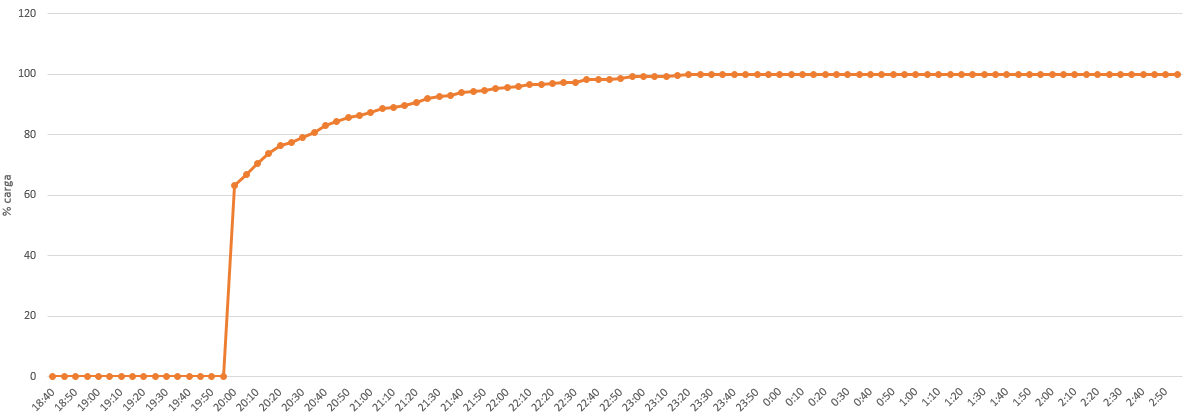
\includegraphics[width=1\textwidth]{fOI0sHj9ac.png}
  \caption{Porcentaje de mesas cargadas}
  \label{graf:porcentajeNeuquen}
\end{figure}

\begin{figure}[h!]
  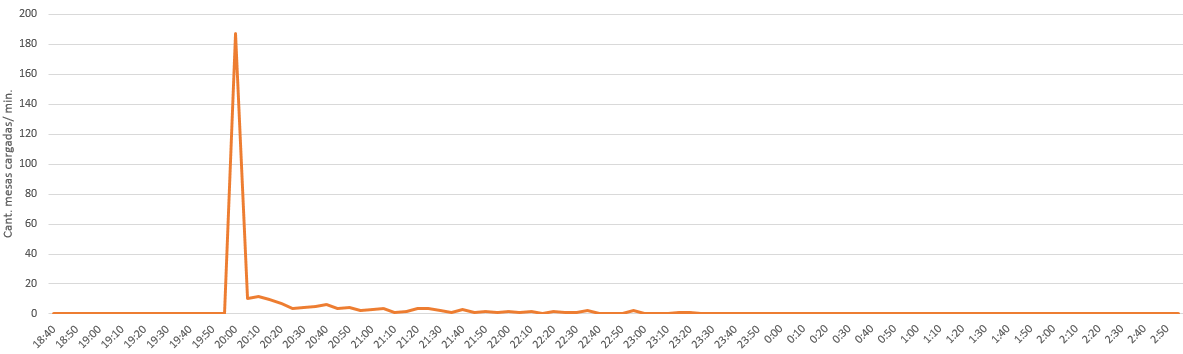
\includegraphics[width=1\textwidth]{QOsSnICbyL.png}
  \caption{Velocidad en carga de mesas}
  \label{graf:velocidadNeuquen}
\end{figure}

\section{Elecciones Rio Negro}
El 7 de Abril de 2019, Río Negro realizó la elección para gobernador y vicegobernador por medio del sistema tradicional de votación en papel. Esto quiere decir que cada votante contendrá en su sobre su lista y/o listas elegida en papel y, el escrutinio se realiza manualmente enviándose los datos desde cada escuela por medio de telegramas. El proceso de votación para esta elección se conformó de los siguientes elementos:
\begin{itemize}
    \item 7 listas candidatas que el elector puede elegir.
    \item 546.067 electores habilitados, esto quiere decir que se preparon 546.000 sobres aproximadamante, uno por cada elector.
    \item 1646 mesas, esto implica la misma cantidad de urnas.
\end{itemize}
Teniendo estos datos se puede concluir que sólo para elecciones de gobernador y vice se utilizaron aprox. 3.822.000 papeles, 7 listas preparadas para 546.000 electores. De igual manera que en las elecciones de Neuquén, se obtuvieron los datos de las elecciones utilizando la técnica de web scraping, obteniendo una evolución de carga de mesas representado en el gráfico \ref{graf:porcentajeRioNegro} y su velocidad de carga en el gráfico \ref{graf:velocidadRioNegro}. Como se puede ver, los datos fueron agrupados en fracciones de 10 min durante todo el proceso de escrutinio.

\begin{figure}[h!]
  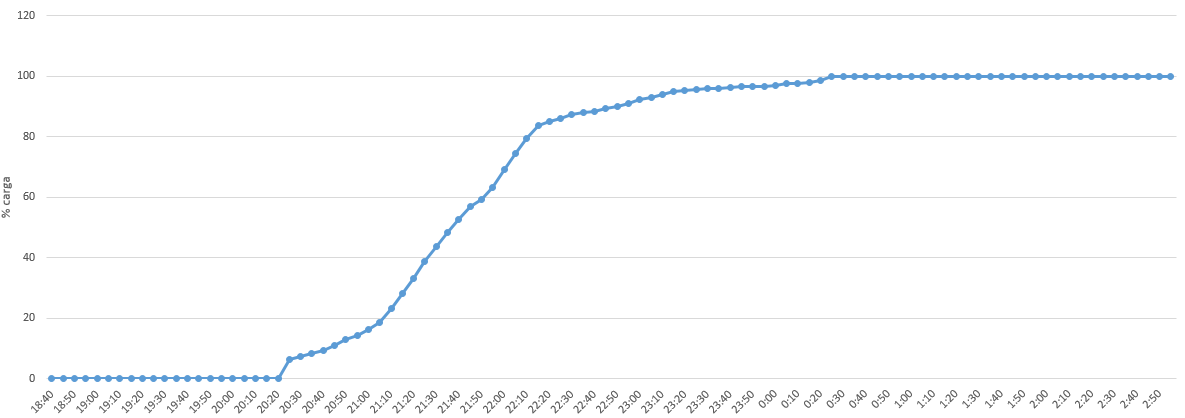
\includegraphics[width=1\textwidth]{sAveHlGEkX.png}
  \caption{Porcentaje de mesas cargadas}
  \label{graf:porcentajeRioNegro}
\end{figure}

\begin{figure}[h!]
  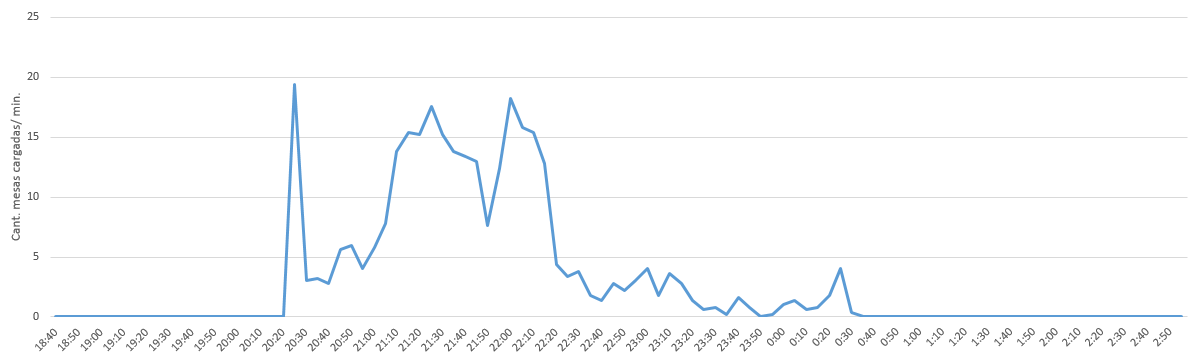
\includegraphics[width=1\textwidth]{8w25IVQD5U.png}
  \caption{Velocidad en carga de mesas}
  \label{graf:velocidadRioNegro}
\end{figure}

\section{Elecciones Córdoba}
El 12 de Mayo de 2019, Córdoba realizó la elección para gobernador, legislador y candidatos a ocupar el tribunal de cuentas provincial y, algunas localidades renovaron autoridades municipales, por medio del sistema de boleta única de sufragio (BUS). Este método consta de una única boleta sobre el cual el votante indica su elección dentro de esta boleta, el cual se ingresa en la urna. Por lo tanto, el sistema consta en imprimir en un único papel todos los cargos y candidatos. En las columnas se organizan cada uno de los cargos y en las filas se listan los espacios políticos como se puede ver en la imagen \ref{graf:BUSCordoba}.
\begin{figure}[h!]
  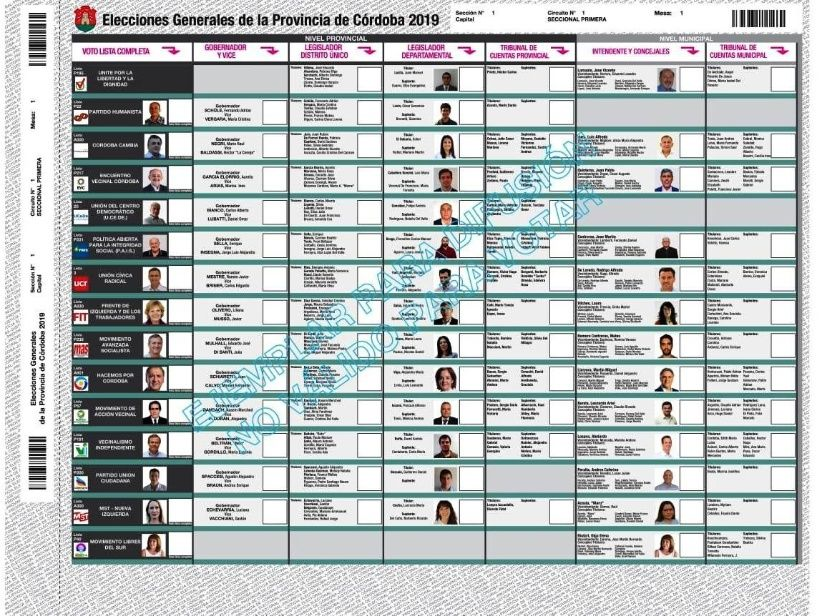
\includegraphics[width=1\textwidth]{boletaunica-cordoba.jpg}
  \caption{Ejemplo de la Boleta Única de Sufragio (BUS)}
  \label{graf:BUSCordoba}
\end{figure}
Luego el escrutinio se realizó de manera manual enviándose los datos de cada escuela por medio de telegramas. El proceso de votación para esta elección se conformó de los siguientes elementos: 
\begin{itemize}
    \item 13 listas candidatas para gobernador que el elector puede elegir
    \item 2.889.973 electores habilitados, esto quiere decir que se prepararon 2.889.000 boletas aproximadamente, uno por cada elector
    \item 8654 mesas
    \item 320 millones de pesos costó este sistema. 
\end{itemize}
Debido a que sólo se utiliza una boleta por elector, se puede concluir que sólo para elecciones de gobernador y vice se utilizaron aprox. 2.889.000 papeles. Como se puede ver su resultado es mucho menor a las elecciones de Rio Negro, aún teniendo éste cerca de un 20\% de electores habilitados a comparación de Córdoba. De igual manera que en las elecciones de Neuquén y Rio Negro, se obtuvieron los datos de las elecciones utilizando la técnica de web scraping, obteniendo una evolución de carga de mesas representado en el gráfico \ref{graf:porcentajeCordoba} y su velocidad de carga en el gráfico \ref{graf:velocidadCordoba}. Como se puede ver, los datos agrupados en fracciones de 10 min. durante todo el proceso de escrutinio.

\begin{figure}[h!]
  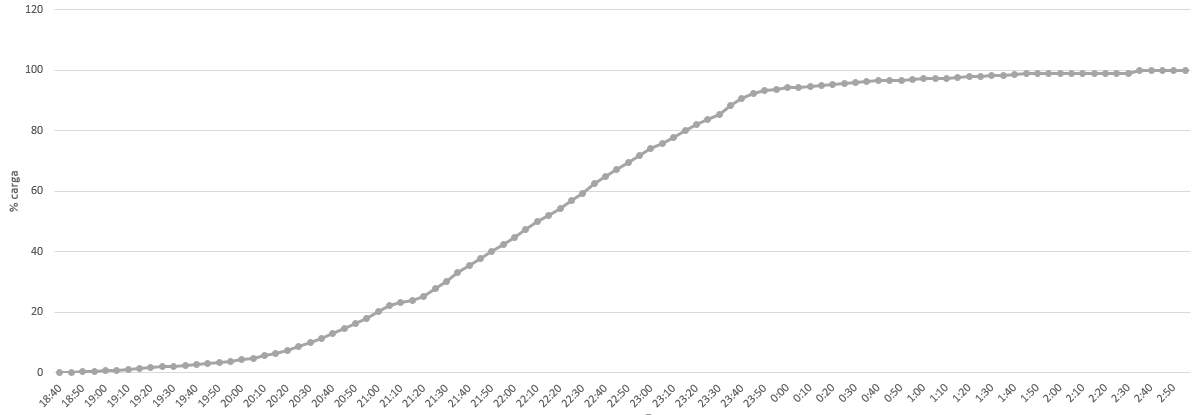
\includegraphics[width=1\textwidth]{E4YqKc5Tcu.png}
  \caption{Porcentaje de mesas cargadas}
  \label{graf:porcentajeCordoba}
\end{figure}

\begin{figure}[h!]
  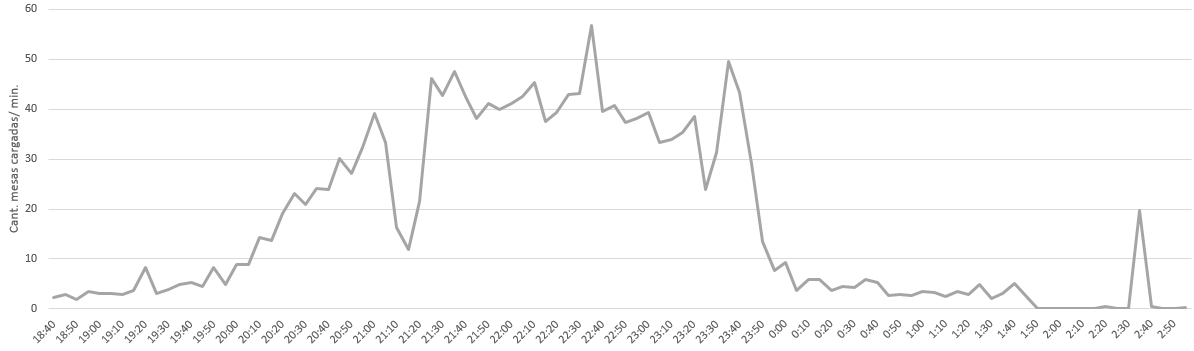
\includegraphics[width=1\textwidth]{9rEiyqeSFw.png}
  \caption{Velocidad en carga de mesas}
  \label{graf:velocidadCordoba}
\end{figure}

\section{Analisis sobre Neuquén, Córdoba y Río Negro}
A través de resultados almacenados en \textit{datosoficiales.com} se consiguieron los datos de cada elección detallada en Neuquén, Rio Negro y Córdoba. \newline
A partir de esto, en el gráfico \ref{fig:velocidad} se puede observar la velocidad comparativa de cada carga en las tres provincias, y en el gráfico \ref{fig:acumulado} se representa el porcentaje acumulado durante el periodo de escrutinio. En estos gráficos, la linea naranja representaría las elecciones utilizando BUE, la linea gris las elecciones utilizando Boleta Única y la linea azul es el resultado de las elecciones tradiciones con boletas partidarias de papel. \newline
A primera impresión se puede observar la notable velocidad de carga en la provincia de Neuquén en los primeros minutos de las 20:00 hs., satisfaciendo el objetivo de rapidez de las máquinas BUE. Sin embargo, se reduce su velocidad hasta completar la totalidad de las mesas. Por otro lado, la provincia de Cordoba, por medio de la Boleta Única logra una velocidad constante de carga hasta completar la totalidad de las mesas. Como se puede observar en el grafico \ref{fig:acumulado} la completitud de las mesas escrutadas se logra con poca diferencia de horas, dando a notar que aplicando tecnología en cualquier etapa del escrutinio no genera un impacto notable en la velocidad de los resultados. 
\newline


\begin{figure}[h!]
  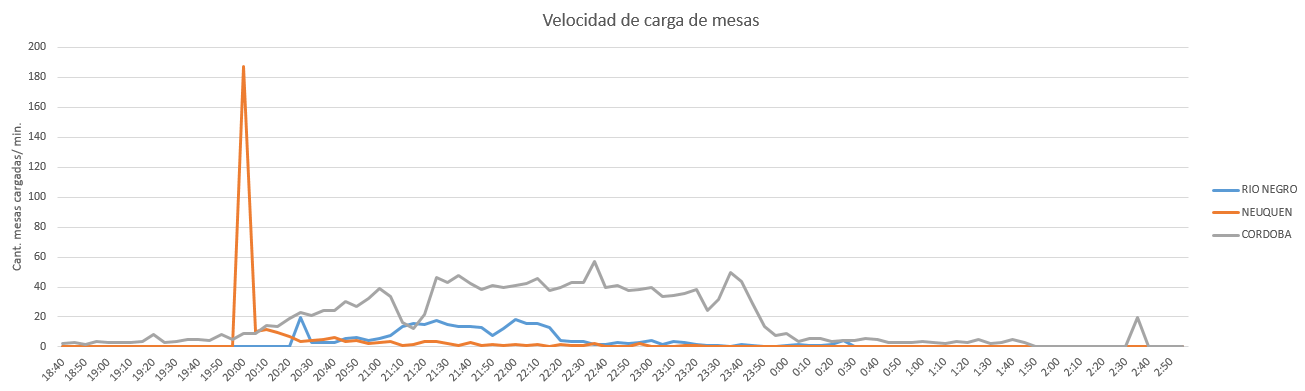
\includegraphics[width=\textwidth]{grafico_velocidad_carga.png}
  \caption{Velocidad de Cargas de mesas}
  \label{fig:velocidad}
\end{figure}
\begin{figure}[h!]
  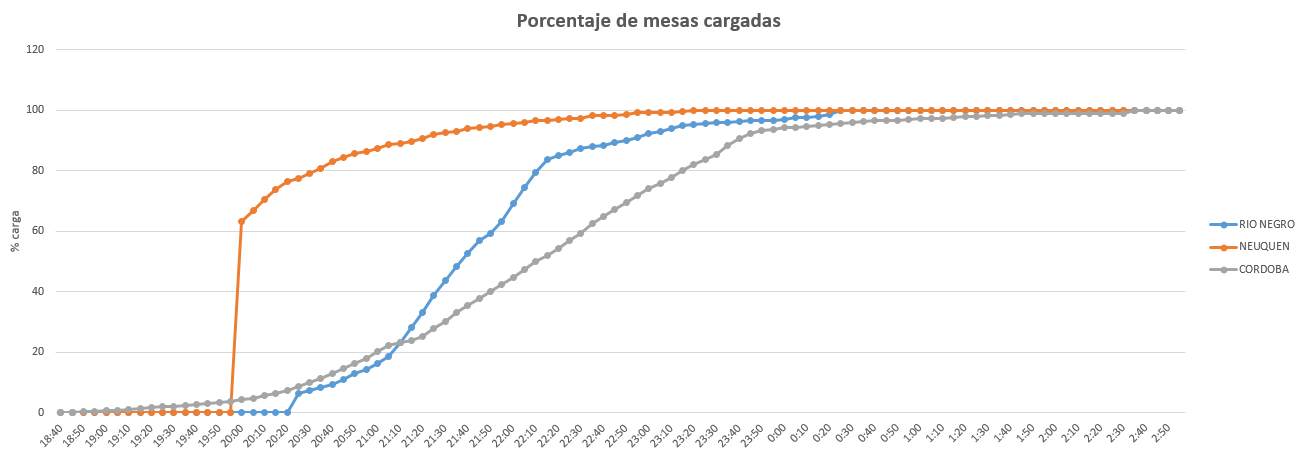
\includegraphics[width=\textwidth]{carga_mesas.png}
  \caption{Porcentaje de mesas cargadas}
  \label{fig:acumulado}
\end{figure}

Otra elección que logró implementar un sistema electoral tradicional sin intervención tecnólogica utilizando la boleta única fue en Bariloche el 1 de Septiembre del 2019 \cite{anbariloche,rnbariloche}. Una característica que que puede generar inconvenientes de este tipo de boleta es el tamaño que puede conseguir, ya que tiene que contener todas las listas disponibles. Por ejemplo, en las elecciones de Córdoba se tiene un tamaño de 40cm de alto por 47 cm de ancho como modelo general, este tamaño podría extenderse en municipios o dependiendo de la cantidad de partidos o alianzas que se presenten \cite{boletaUnicaTamanio}. \newline
Por otra parte, el sistema BUE consta de una boleta con un chif RFID sobre la cual se escribe la voluntad del votante. Dentro del modelo de referencia consta de las fases de Emisión del voto y además esta boleta es utilizada para la fase posterior de Escrutinio de la mesa. A pesar del debate impulsado por varias instituciones en contra del uso de este método, varios municipios lo utilizaron. Un inconveniente que puede albergar este sistema es la limitación en pantalla. Una pantalla dipone de 18 pixeles para ubicar a los candidatos. Con el uso de listas colectoras se llegaron a multiplicar las listas. La disposición de los candidatos en la pantalla de estas máquinas puede afectar la accesibilidad de los electores al reducirse el tamaño de cada cuadricula. Como ejemplo, en Plottier \cite{lmncolectoras} se dispusieron 29 candidatos a intendencia de la ciudad y 26 en Neuquén. 

\section{Opinión sobre las elecciones en Neuquén Capital}
En las elecciones a intendente en Neuquén Capital el día 22 de Septiembre de 2019 se realizó una encuesta con la intención de conocer las opiniones de los votantes. Al ser un municipio que luego de 4 elecciones utilizando el sistema BUE, sería una buena muestra de votantes con experiencia sobre este dispositivo, o es lo que se espera. Esta actividad involucró votantes de cuatro escuelas repartidas en puntos importantes de la ciudad. Las escuelas encuestadas fueron Esc. nº201 (Barrio Centro), nº 40 (Barrio San Lorenzo), nº 20 (Barrio Don Bosco) y nº 103 (Barrio Confluencia) logrando encuestar 145 personas en total. \newline
El objetivo de esta encuesta fue conocer el nivel de aprendizaje de los votantes sobre este nuevo sistema y en respuesta a su uso, cuánta confianza y facilidad les resulta este medio de votación. A cada votante se le hacian cinco preguntas con opciones de respuesta para que el cuestionario se logre hacer en no más de 5 minutos. Las preguntas fueron:
\begin{enumerate}
    \item ¿La persona encuestada votó?
    \item ¿La persona encuestada leyó su boleta impresa?
    \item ¿La persona encuestada verificó su boleta utilizando el lector de chip RFID?
    \item ¿A la persona encuestada le resulta simple votar con la boleta BUE?
    \item ¿La persona encuestada confía en el sistema de votación utilizada?
\end{enumerate}

Cabe aclarar que esta encuesta se realizó a 100 metros de distancia de la escuela por Código Electoral y como se puede observar las preguntas estaban enfocadas a cómo realizar la votación, no se hicieron preguntas personales sobre su voto. Se decidió subdividir las muestras por edad generacional, por lo tanto, se encuadra cada votante dentro de las categorias
\begin{itemize}
    \item Z: Personas nacidas a partir del 2000, representado en la tabla como menores a 25 años aprox.
    \item Y: Personas nacidas entre 1980-1999, representado en la tabla con edades entre 25 y 39 años aprox.
    \item X: Personas nacidas entre 1965-1979, representado en la tabla con edades entre 39 y 55 años aprox.
    \item BG: Personas nacidas entre 1946-1964, representado en la tabla con edades mayores a 55 años aprox.
\end{itemize}
Al finalizar las encuestas se obtuvieron los datos de la tabla \ref{tab:encuesta} donde se contabilizan la cantidad de personas que respondieron a cada opción para cada pregunta.
\begin{table}[h!]
\caption{Resultado sobre los encuestados}
\begin{center}
\resizebox{\textwidth}{!}{
\begin{tabular}{ |c|c|||c|c|c||c|c|c||c|c|c||c|c|c|c| } 
 \hline
 \multirow{2}{4em}{Pregunta} & \multirow{2}{3em}{Generación} & \multicolumn{3}{|c||}{Escuela nº201} & \multicolumn{3}{|c||}{Escuela nº40} & \multicolumn{3}{|c||}{Escuela nº20} & \multicolumn{3}{|c|}{Escuela nº103} & \multirow{2}{3em}{Total}\\
  & &SI & MASO & NO & SI & MASO & NO & SI & MASO & NO & SI & MASO & NO & \\ 
 \hline
 \multirow{4}{3em}{¿Votó?} & Z < 25 & 2 & & & 7 & & & 4 & & & 5 & & & 18 \\ 
 & 25 <= Y < 39 & 8 & & & 12 & & & 12 & & & 4 & & & 36\\ 
 & 39 <= X < 55 & 15 & & & 12 & & & 13 & & & 23 & & & 63 \\
 & 55 <= BG & 12 & & & 5 & & & 7 & & & 4 & & & 28\\ 
 \hline \hline
 \multirow{4}{3em}{¿Leyó?} & Z < 25 & 1 & & 1 & 6 & & 1 & 4 & & & 5 & & & 18\\ 
 & 25 <= Y < 39 & 8 & & & 11 & & 1 & 11 & & 1 & 4 & & & 36\\ 
 & 39 <= X < 55 & 15 & & & 9 & & 3 & 11 & & 2 & 20 & & 3 & 63 \\
 & 55 <= BG & 11 & & 1 & 3 & & 2 & 7 & & & 3 & & 1 & 28 \\ 
 \hline \hline
 \multirow{4}{3em}{¿Verificó?} & Z < 25 &  & & 2 & 6 & & 1 & 1 & & 3 & 4 & & 1 & 18 \\ 
 & 25 <= Y < 39 & 5 & & 3 & 4 & & 7 & 8 & & 4 & 3 & & 1 & 36\\ 
 & 39 <= X < 55 & 8 & & 7 & 7 & & 6 & 4 & & 9 & 14 & & 9 & 63 \\
 & 55 <= BG & 5 & & 7 & 4 & & 1 & 4 & & 3 & 3 & & 1 & 28\\ 
 \hline \hline
 \multirow{4}{3em}{¿Es simple?} & Z < 25 & 2 & & & 6 & 1 & & 4 & & & 5 & & & 18 \\ 
 & 25 <= Y < 39 & 8 & & & 11 & & & 11 & 1 & & 4 & & & 35 \\ 
 & 39 <= X < 55 & 14 & & 1 & 12 & 1 & & 11 & 1 & 1 & 21 & 2 & & 64 \\
 & 55 <= BG & 12 & & & 3 & & 2 & 6 & & 1 & 2 & & 2 & 28 \\ 
 \hline \hline
 \multirow{4}{3em}{¿Confía?} & Z < 25 & 2 & & & 3 & & 4 & 1 & & 3 & 3 & 2 & & 18 \\ 
 & 25 <= Y < 39 & 4 & 3 & 1 & 1 & 4 & 6 & 6 & 1 & 5 & 1 & 1 & 2 & 33 \\ 
 & 39 <= X < 55 & 10 & 3 & 2 & 4 & 3 & 6 & 8 & 2 & 3 & 14 & 6 & 3 & 64\\
 & 55 <= BG & 10 & 2 & & & 1 & 4 & 3 & & 4 & 2 & & 2 & 28\\ 
 \hline \hline
\end{tabular}
}
\label{tab:encuesta}
\end{center}
\end{table}

Teniendo los datos finales, se logra ver una gran cantidad de personas que leen sus boletas impresas pero no asi con la lectura del chip integrado en la boleta, como se observa en el gráfico \ref{graf:votantes}. A pesar de haber experimentado este sistema en distintas elecciones se descubrió que muchos de ellos no sabian la existencia del lector de chip, dato que no se esperaba. Como se puede ver en el gráfico cerca del 50\% desconocía esta verificación y no varía según la edad generacional.

\begin{figure}[h!]
  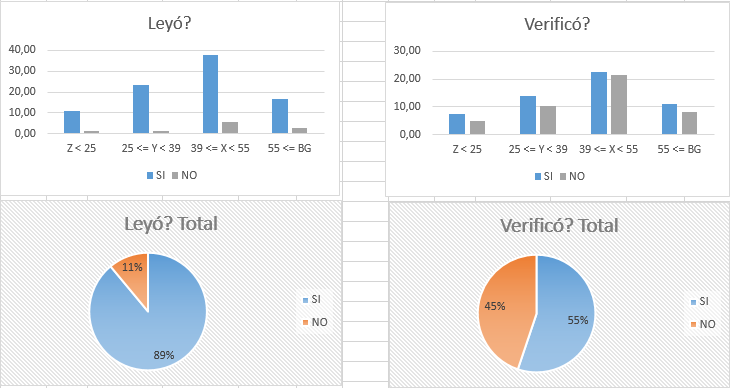
\includegraphics[width=\textwidth]{yfrjnCosp0.png}
  \caption{Comparación entre los que leen y verifican su boleta electrónica}
  \label{graf:votantes}
\end{figure}

Otro dato curioso de estas opiniones es que casi la totalidad de las personas les resulta sencillo su uso, sin embargo, muy pocas de ellas les genera confianza. Como se puede ver en el gráfico \ref{graf:votantesUsoConfia} la mitad de los encuestados les genera confianza o intentan confiar en este sistema. Sobre esta última característica destaca la variación de opiniones según la zona urbana encuestada, como se puede ver en la tabla, en el área centro se concentra la cantidad de personas que aprueban sistema BUE, seguido del área Confluencia. Por otro lado las demás áreas no logran confiar en este sistema. 
\begin{figure}[h!]
  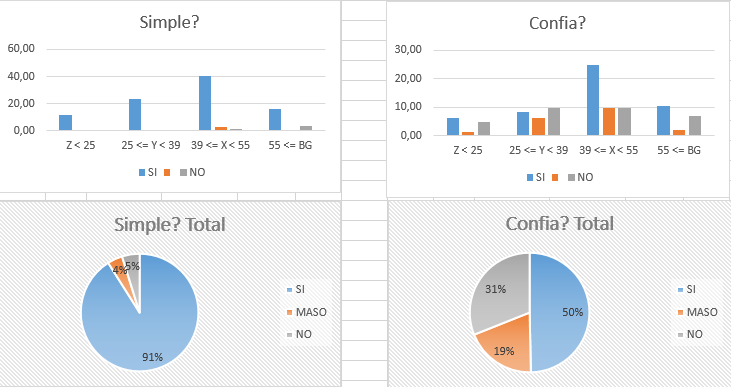
\includegraphics[width=\textwidth]{SLLXOorTia.png}
  \caption{Usabilidad vs. Confiabilidad}
  \label{graf:votantesUsoConfia}
\end{figure}

\section{Sistema Escrutinio Nacional 2019}
En 2019 se utiliza el sistema llamado SmartTally \cite{smartally} , que consta en el envio de telegramas directo desde el establecimiento hacia los centros de cómputos de la Dirección Nacional Electoral (DINE), que depende del Ministerio del Interior de la Nación. Con el objeto de agilizar el trámite que es llevado a cabo por el Correo Argentino. Cada establecimiento consta de una impresora multifunción, conexión a internet y un equipo que permite la conexión y monitoreo del envio exitoso de los telegramas. \newline
Este sistema fue usado en las elecciones las PASO (11 de Agosto de 2019) y Elecciones Naciones (27 de Octubre de 2019). Toda documentación de capacitación se encuentra disponible en una carpeta compartida \cite{manualesCorreoArg}.\newline
Polémicas al usar este tipo de sistema:
\begin{itemize}
    \item Auditabilidad del Software: Se requirió que la empresa ponga a disponibilidad el software usado para su investigación, a modo de reconocer posibles fallas. Frente a este pedido el Gobierno notifica que no es posible ya que el software es alquilado y la empresa dueña se niega a entregar este producto.\cite{auditabilidadSmartmatic}
    \item Seguridad frente a ataques externos: Javier Smaldone presentó vulnerabilidades en el software de conversión de formato de los \"telegramas\" electorales poniendo en riesgo la integridad del proceso. \cite{seguridadSmartmatic}
    \item Transparencia: Debido a que este sistema consta de dos etapas en el proceso de escrutinio, existe cierta desconfianza entre los datos cargados por cada transmisión exponiendo los resultados provisorios y el resultado final luego de ser validado dentro de los 10 días como indica el código electoral. Este primer resultado podría generar datos ganadores que luego no son así en el resultado final. \cite{rnEscrutinioProvisorio}
\end{itemize}
